\newpage

\section{More Circles}

\begin{teachingnote}
This first problem is very difficult because students have to draw pictures that are clearly wrong.  Pick and choose from among the remaining problems, which might benefit from scaffolding to make them more ``activity like.''
\end{teachingnote}

\fixnote{The first problem is made considerably easier by first proving that the shortest distance from a point to a line is along a perpendicular.  That is proven indirectly.  Then Problem 1 is pretty straightforward from the definition of a circle as the set of points that are equidistant from a center.  All other points on the line must be a greater distance from the center.}

\begin{prob}
Prove: The radius of a circle is perpendicular to the tangent where the radius intersects the circle.  Hint:  Suppose not. 
\end{prob}

\begin{prob}
Suppose an angle circumscribes a circle, as shown below.  Find a relationship between the measure of the angle and the measure of the central angle intercepted by the same chord.
$$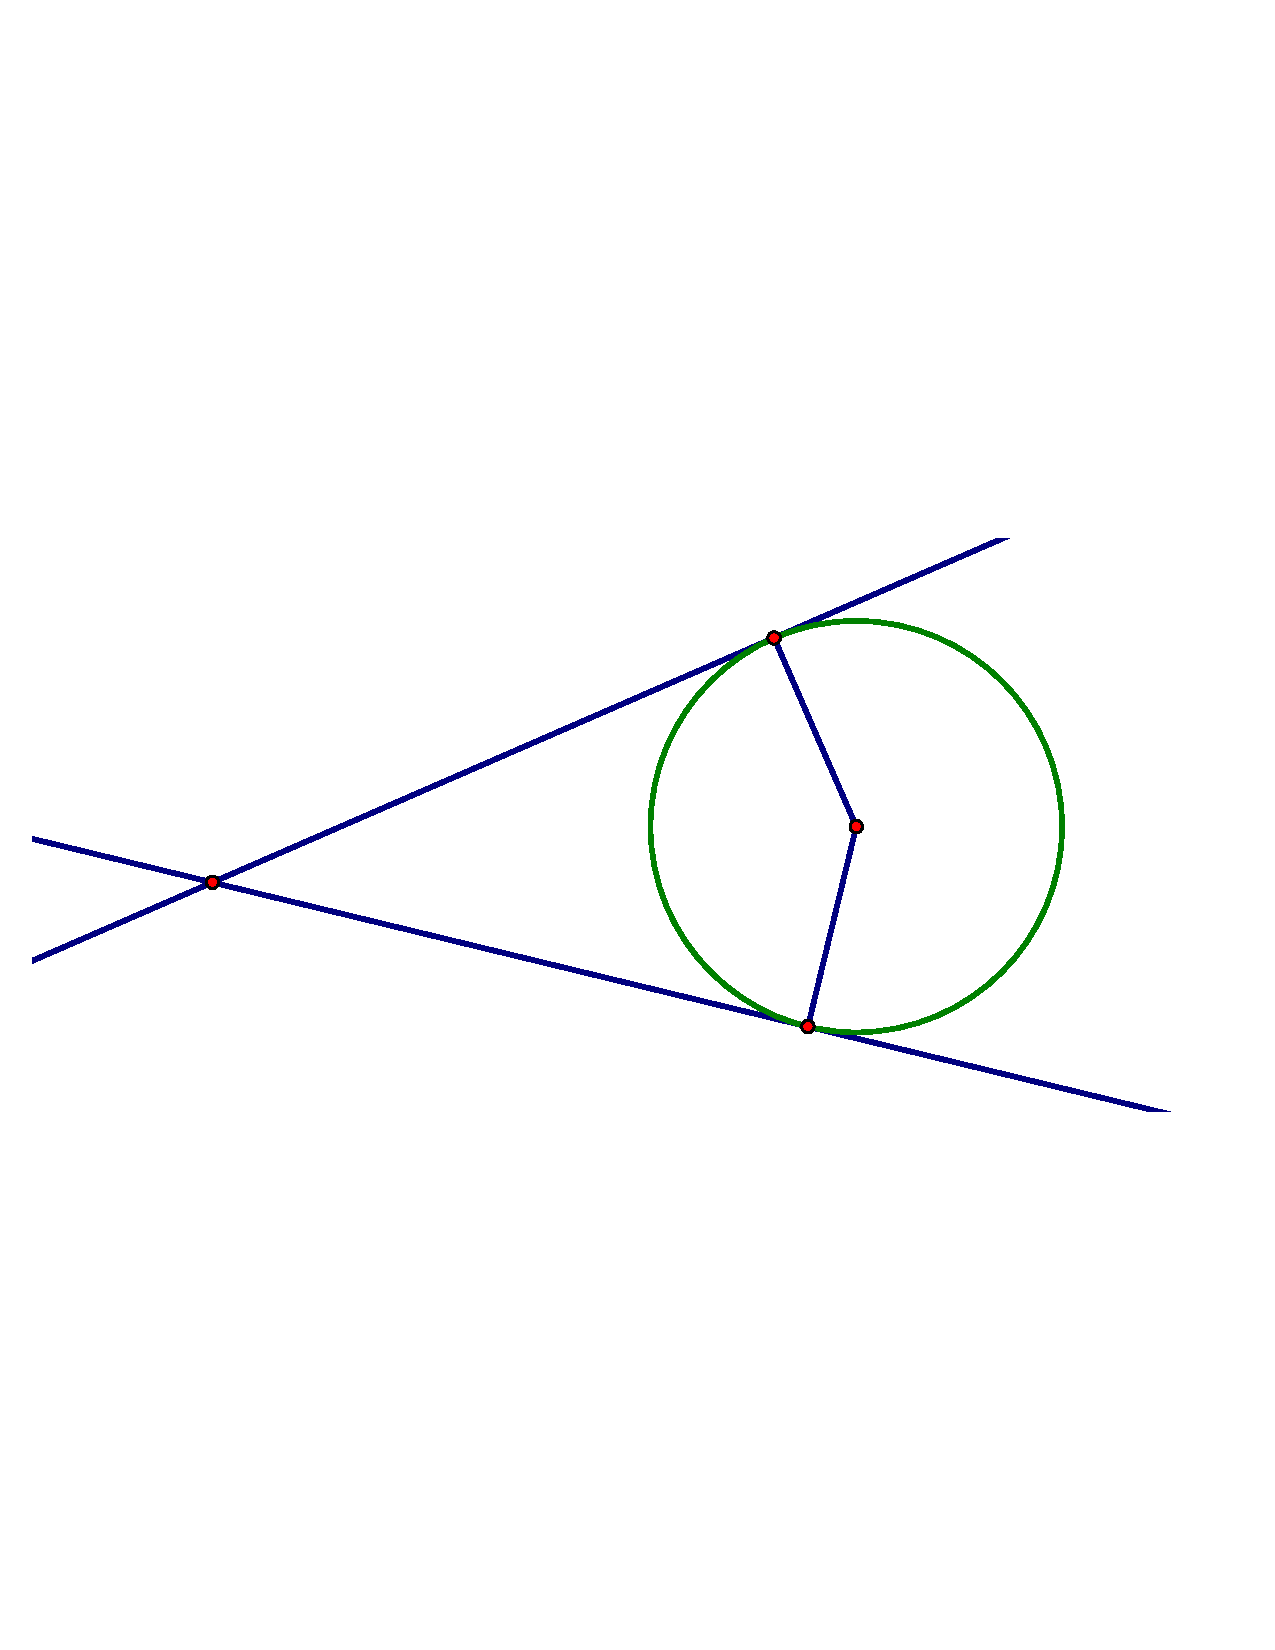
\includegraphics[width=2.5in]{../graphics/circumscribedAngle.pdf}$$
\end{prob}

\begin{prob}
Show that, given any three non-collinear points in the Euclidean
plane, there is a unique circle passing through the three points.
\end{prob}

\begin{prob}
Draw four points in the Euclidean plane, no three of which are collinear, that cannot lie on a single circle.  Explain your reasoning. 
\end{prob}

\begin{prob}
Using a compass, draw a large circle, and inscribe a quadrilateral in the circle.  Measure the four angles.  Repeat with another circle and quadrilateral.  What do you notice?  Identify a condition on any quadrilateral that is inscribed in a circle.  Now prove it.  
\end{prob}

\begin{prob}
Construct a tangent line to a circle from a point outside the given circle.
$$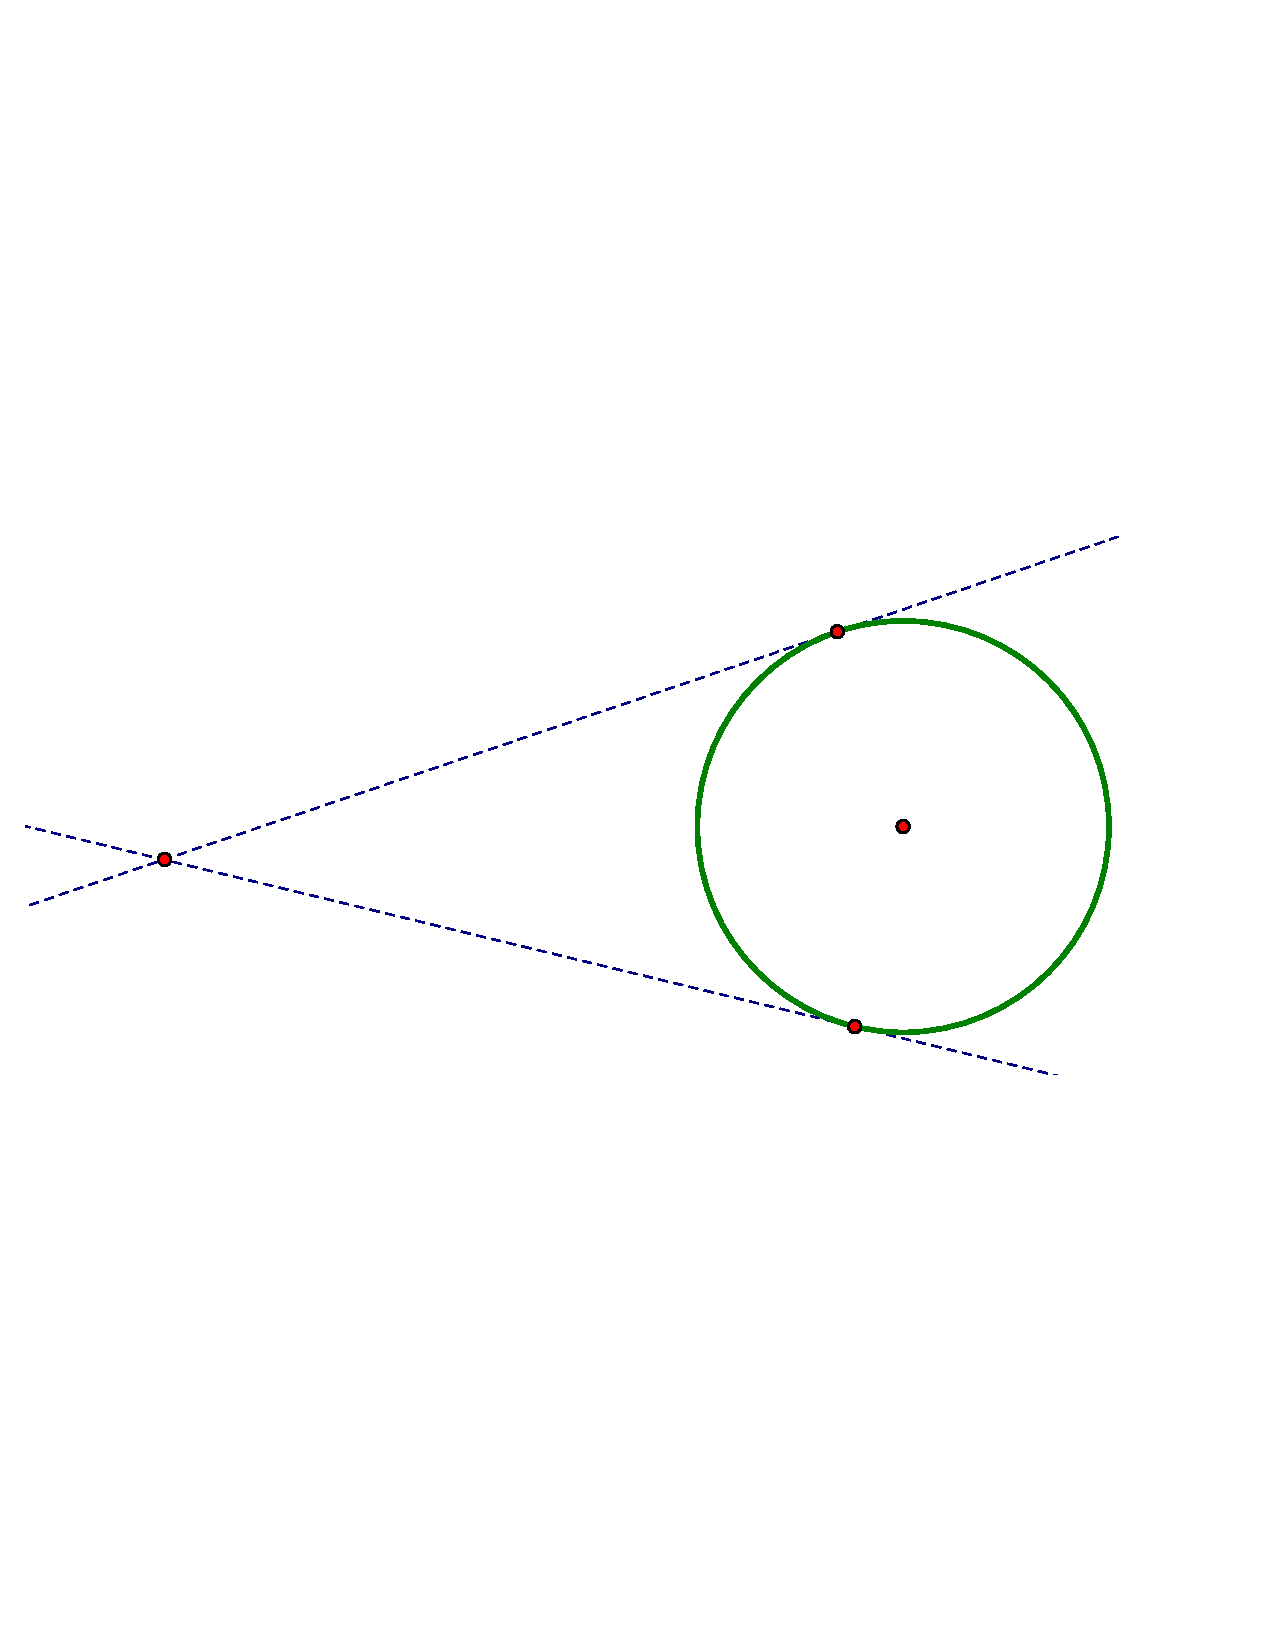
\includegraphics[width=3in]{../graphics/tangent2.pdf}$$
\end{prob}

\begin{prob}
Give an informal derivation of the relationship between the circumference and area of a circle.  Imagine cutting a circle into ``pie pieces'' and rearranging the pieces into a shape like the one below.  As the circle is cut into more and more equal-sized ``pie pieces,'' what does the rearranged shape begin to resemble?  Can you find the area of this shape?  
$$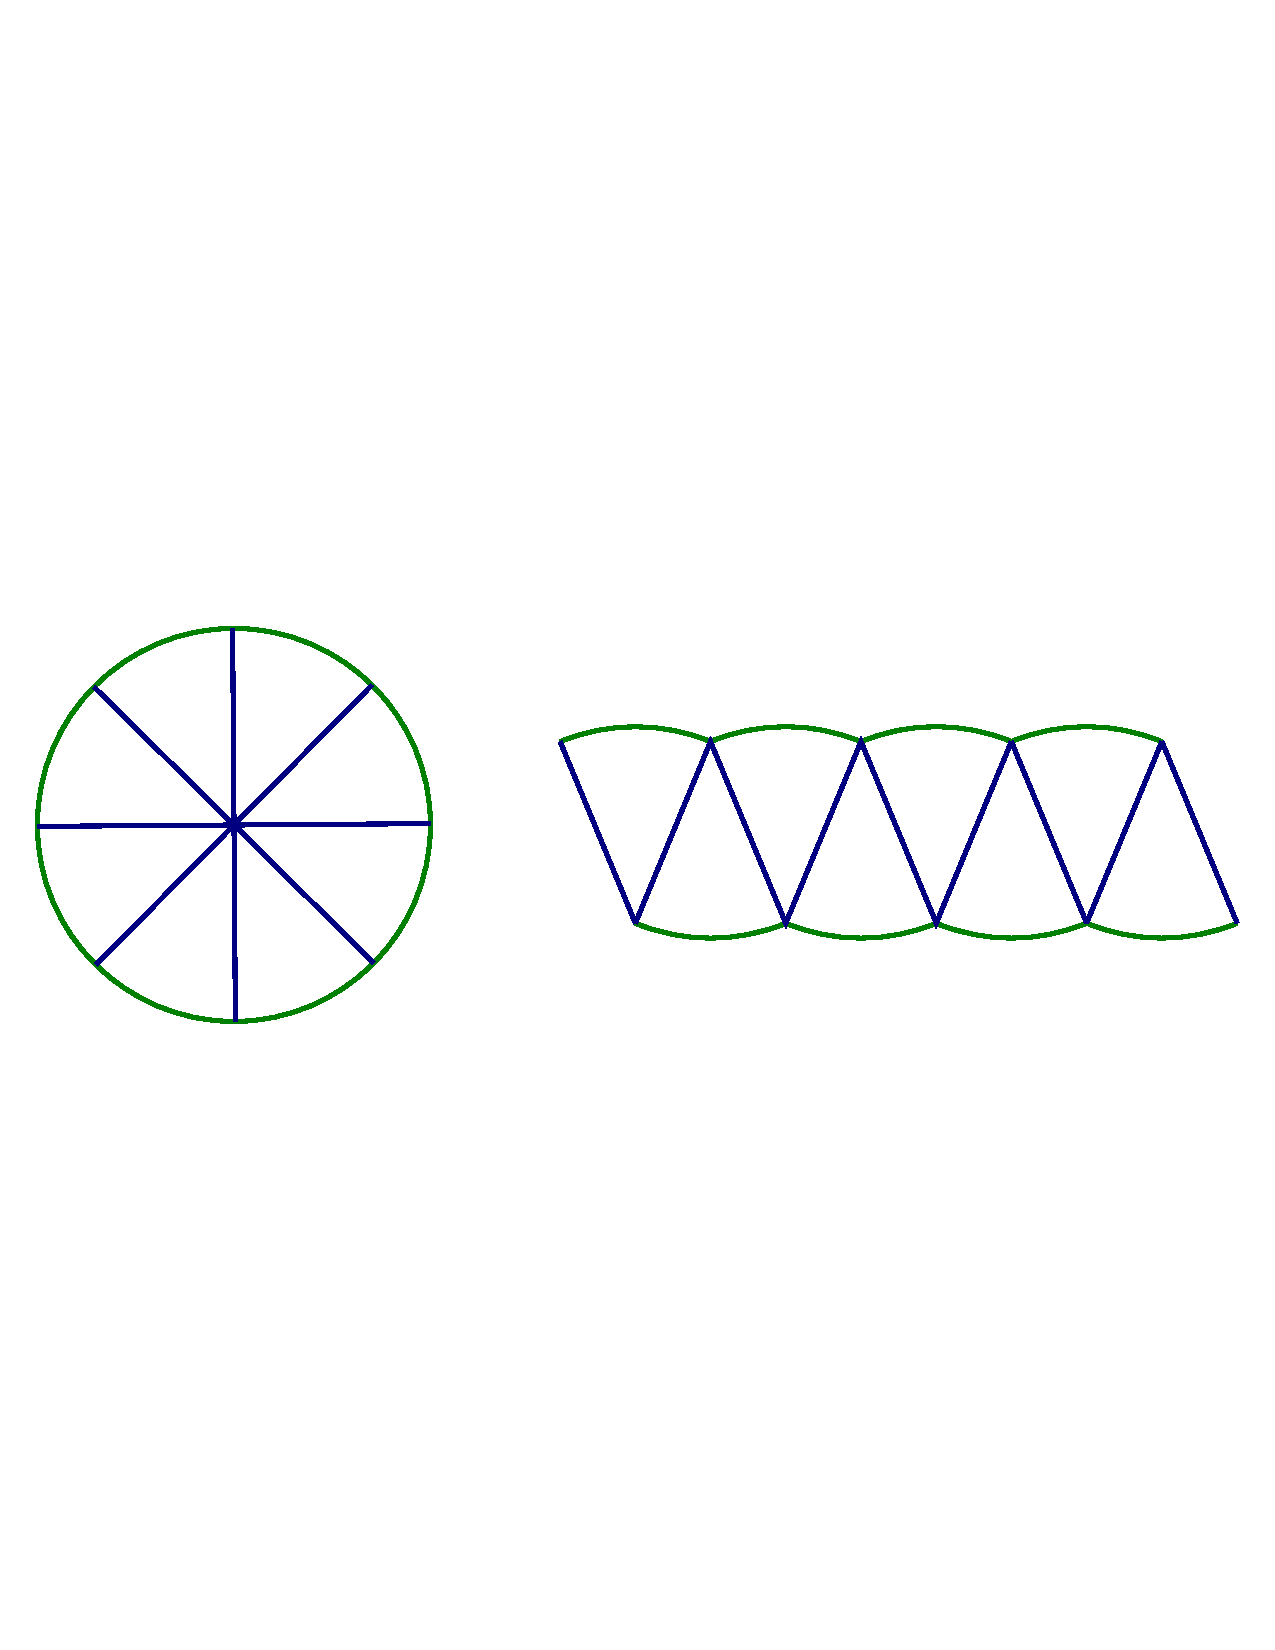
\includegraphics[width=3.5in]{../graphics/circleArea.pdf}$$
\end{prob}

\begin{prob}
Derive a formula for the length of the arc intercepted by an central angle of a circle.  
\end{prob}

\begin{prob}
Derive a formula for the area of a sector of a circle.  
\end{prob}

%\begin{prob}
%Explain the following statement:  Given a central angle of a circle, the length of the intercepted arc is proportional to the radius of the circle.  The radian measure of the angle is the constant of proportionality.  (Hint:  Illustrate your explanation with a familiar angle.)
%\end{prob}

